% BASIC SETTINGS
\documentclass[a4paper,12pt]{article} % Set paper size and document type
\usepackage{lmodern} % Use a slightly nicer looking font
\usepackage{url} % Proper formatting for URLs
\usepackage{graphicx} % Handle inclusion of non-PDF graphics
\usepackage{subfig} % Allow sub-figures inside a figure
\usepackage{enumitem} % Allow lists to pick up numbering where the last list left off

% Change margins - default margins are too broad
\usepackage[margin=20mm]{geometry}

% SOURCE CODE LISTING SETTINGS 
% https://en.wikibooks.org/wiki/LaTeX/Source_Code_Listings
\usepackage{listings}
\usepackage{color}

% Color definitions for source code listings
\definecolor{mygreen}{rgb}{0,0.6,0}
\definecolor{mygray}{rgb}{0.5,0.5,0.5}
\definecolor{mymauve}{rgb}{0.58,0,0.82}

% Formatting (line breaks, spacing, etc...) for code
\lstset{ 
  backgroundcolor=\color{white},   % choose the background color; you must add \usepackage{color} or \usepackage{xcolor}
  basicstyle=\footnotesize,        % the size of the fonts that are used for the code
  breakatwhitespace=false,         % sets if automatic breaks should only happen at whitespace
  breaklines=true,                 % sets automatic line breaking
  captionpos=b,                    % sets the caption-position to bottom
  commentstyle=\color{mygreen},    % comment style
  deletekeywords={...},            % if you want to delete keywords from the given language
  escapeinside={\%*}{*)},          % if you want to add LaTeX within your code
  extendedchars=true,              % lets you use non-ASCII characters; for 8-bits encodings only, does not work with UTF-8
  frame=single,	                   % adds a frame around the code
  keepspaces=true,                 % keeps spaces in text, useful for keeping indentation of code (possibly needs columns=flexible)
  keywordstyle=\color{blue},       % keyword style
  otherkeywords={*,...},           % if you want to add more keywords to the set
  numbers=left,                    % where to put the line-numbers; possible values are (none, left, right)
  numbersep=5pt,                   % how far the line-numbers are from the code
  numberstyle=\tiny\color{mygray}, % the style that is used for the line-numbers
  rulecolor=\color{black},         % if not set, the frame-color may be changed on line-breaks within not-black text (e.g. comments (green here))
  showspaces=false,                % show spaces everywhere adding particular underscores; it overrides 'showstringspaces'
  showstringspaces=false,          % underline spaces within strings only
  showtabs=false,                  % show tabs within strings adding particular underscores
  stepnumber=2,                    % the step between two line-numbers. If it's 1, each line will be numbered
  stringstyle=\color{mymauve},     % string literal style
  tabsize=2,	                   % sets default tabsize to 2 spaces
  title=\lstname                   % show the filename of files included with \lstinputlisting; also try caption instead of title
}

% Set document title and author
\title{\LaTeX \space{} Example \#1}
\author{Jeremy Pedersen}
\date{2022-12-19} % If date is left blank, it will be hidden

% Document body
\begin{document}

\maketitle % Insert the title, author, and date

\section{First section} %  Create a section

We can use the listing package to place source code into our documents from a file:

% Include code from a file with filename indicated
\vspace{5mm}
\lstinputlisting[language=Python]{test_code.py}
\vspace{5mm}

\noindent
Or we can quote a range of line numbers from the file (lines 19 and 20, for example):

% Include only specific lines from a file
\vspace{5mm}
\lstinputlisting[language=Python, firstline=19, lastline=20]{test_code.py}
\vspace{5mm}

% Forces content onto the next page, useful for documents which should look nice when printed out
\clearpage

\noindent
We can also place code directly into latex without importing it from a file:

% Include code inline
\vspace{5mm}
\begin{lstlisting}[language=Python]
print("Hi, I'm Python 3!")
\end{lstlisting}
\vspace{5mm}

\subsection{First subsection} % Create a subsection

We can create and format mathematical expressions like so:

\vspace{2mm}
% Format a mathematical expression
$$x' = x \cdot s cos \theta - y \cdot s sin \theta + t_x$$
$$y' = x \cdot s sin \theta + y \cdot s cos \theta + t_y$$
\vspace{2mm}

\noindent
We can also make a nice list:

% Make a list
\vspace{2mm}
\begin{enumerate}
\item I am the first thing in the list
\item I am the second thing in the list
\end{enumerate}
\vspace{2mm}

\noindent
We can inline mathematical expressions such as this one "$4 \sigma_0$" using the "\$" sign. We can make mathematical expressions that occupy their own line, like this: 
\vspace{2mm}
$$u = (x - x_0) \frac{1}{4 \sigma_0} cos \theta_0 - (y - y_0) \frac{1}{4 \sigma_0} sin \theta_0 + 4 = (0 - 16) \frac{1}{4} - 0 + 4$$
\vspace{2mm}

\subsection{Second subsection}

We can also make tables and charts using the array type like so:

% Make an array or table
\vspace{2mm}
\[ \phi = \left\{ 
\begin{array}{l l}
\theta_0 + \theta_{pt} & if \ \theta_0 + \theta_{pt} \in [0,2 \pi)\\ 
\theta_0 + \theta_{pt} + 2 \pi & if \ \theta_0 + \theta_{pt} < 0\\
\theta_0 + \theta_{pt} - 2 \pi & if \ \theta_0 + \theta_{pt} \ge 2 \pi\\
\end{array} \right\}
\] 
\vspace{2mm}

\noindent
I can start an enumerated list of items here...

\vspace{5mm}
\begin{enumerate}
\item One thing
\item Another thing
\end{enumerate}
\vspace{5mm}

\noindent
And then...

\section{Second section}

...I can continue it here!

\vspace{5mm}
\begin{enumerate}[resume]
\item Yet more stuff
\item Some other things
\end{enumerate}
\vspace{5mm}

Inserting figures is also relatively easy to do: 

\vspace{5mm}
% Insert a figure with an image
\begin{figure}[!ht]
  \centering
  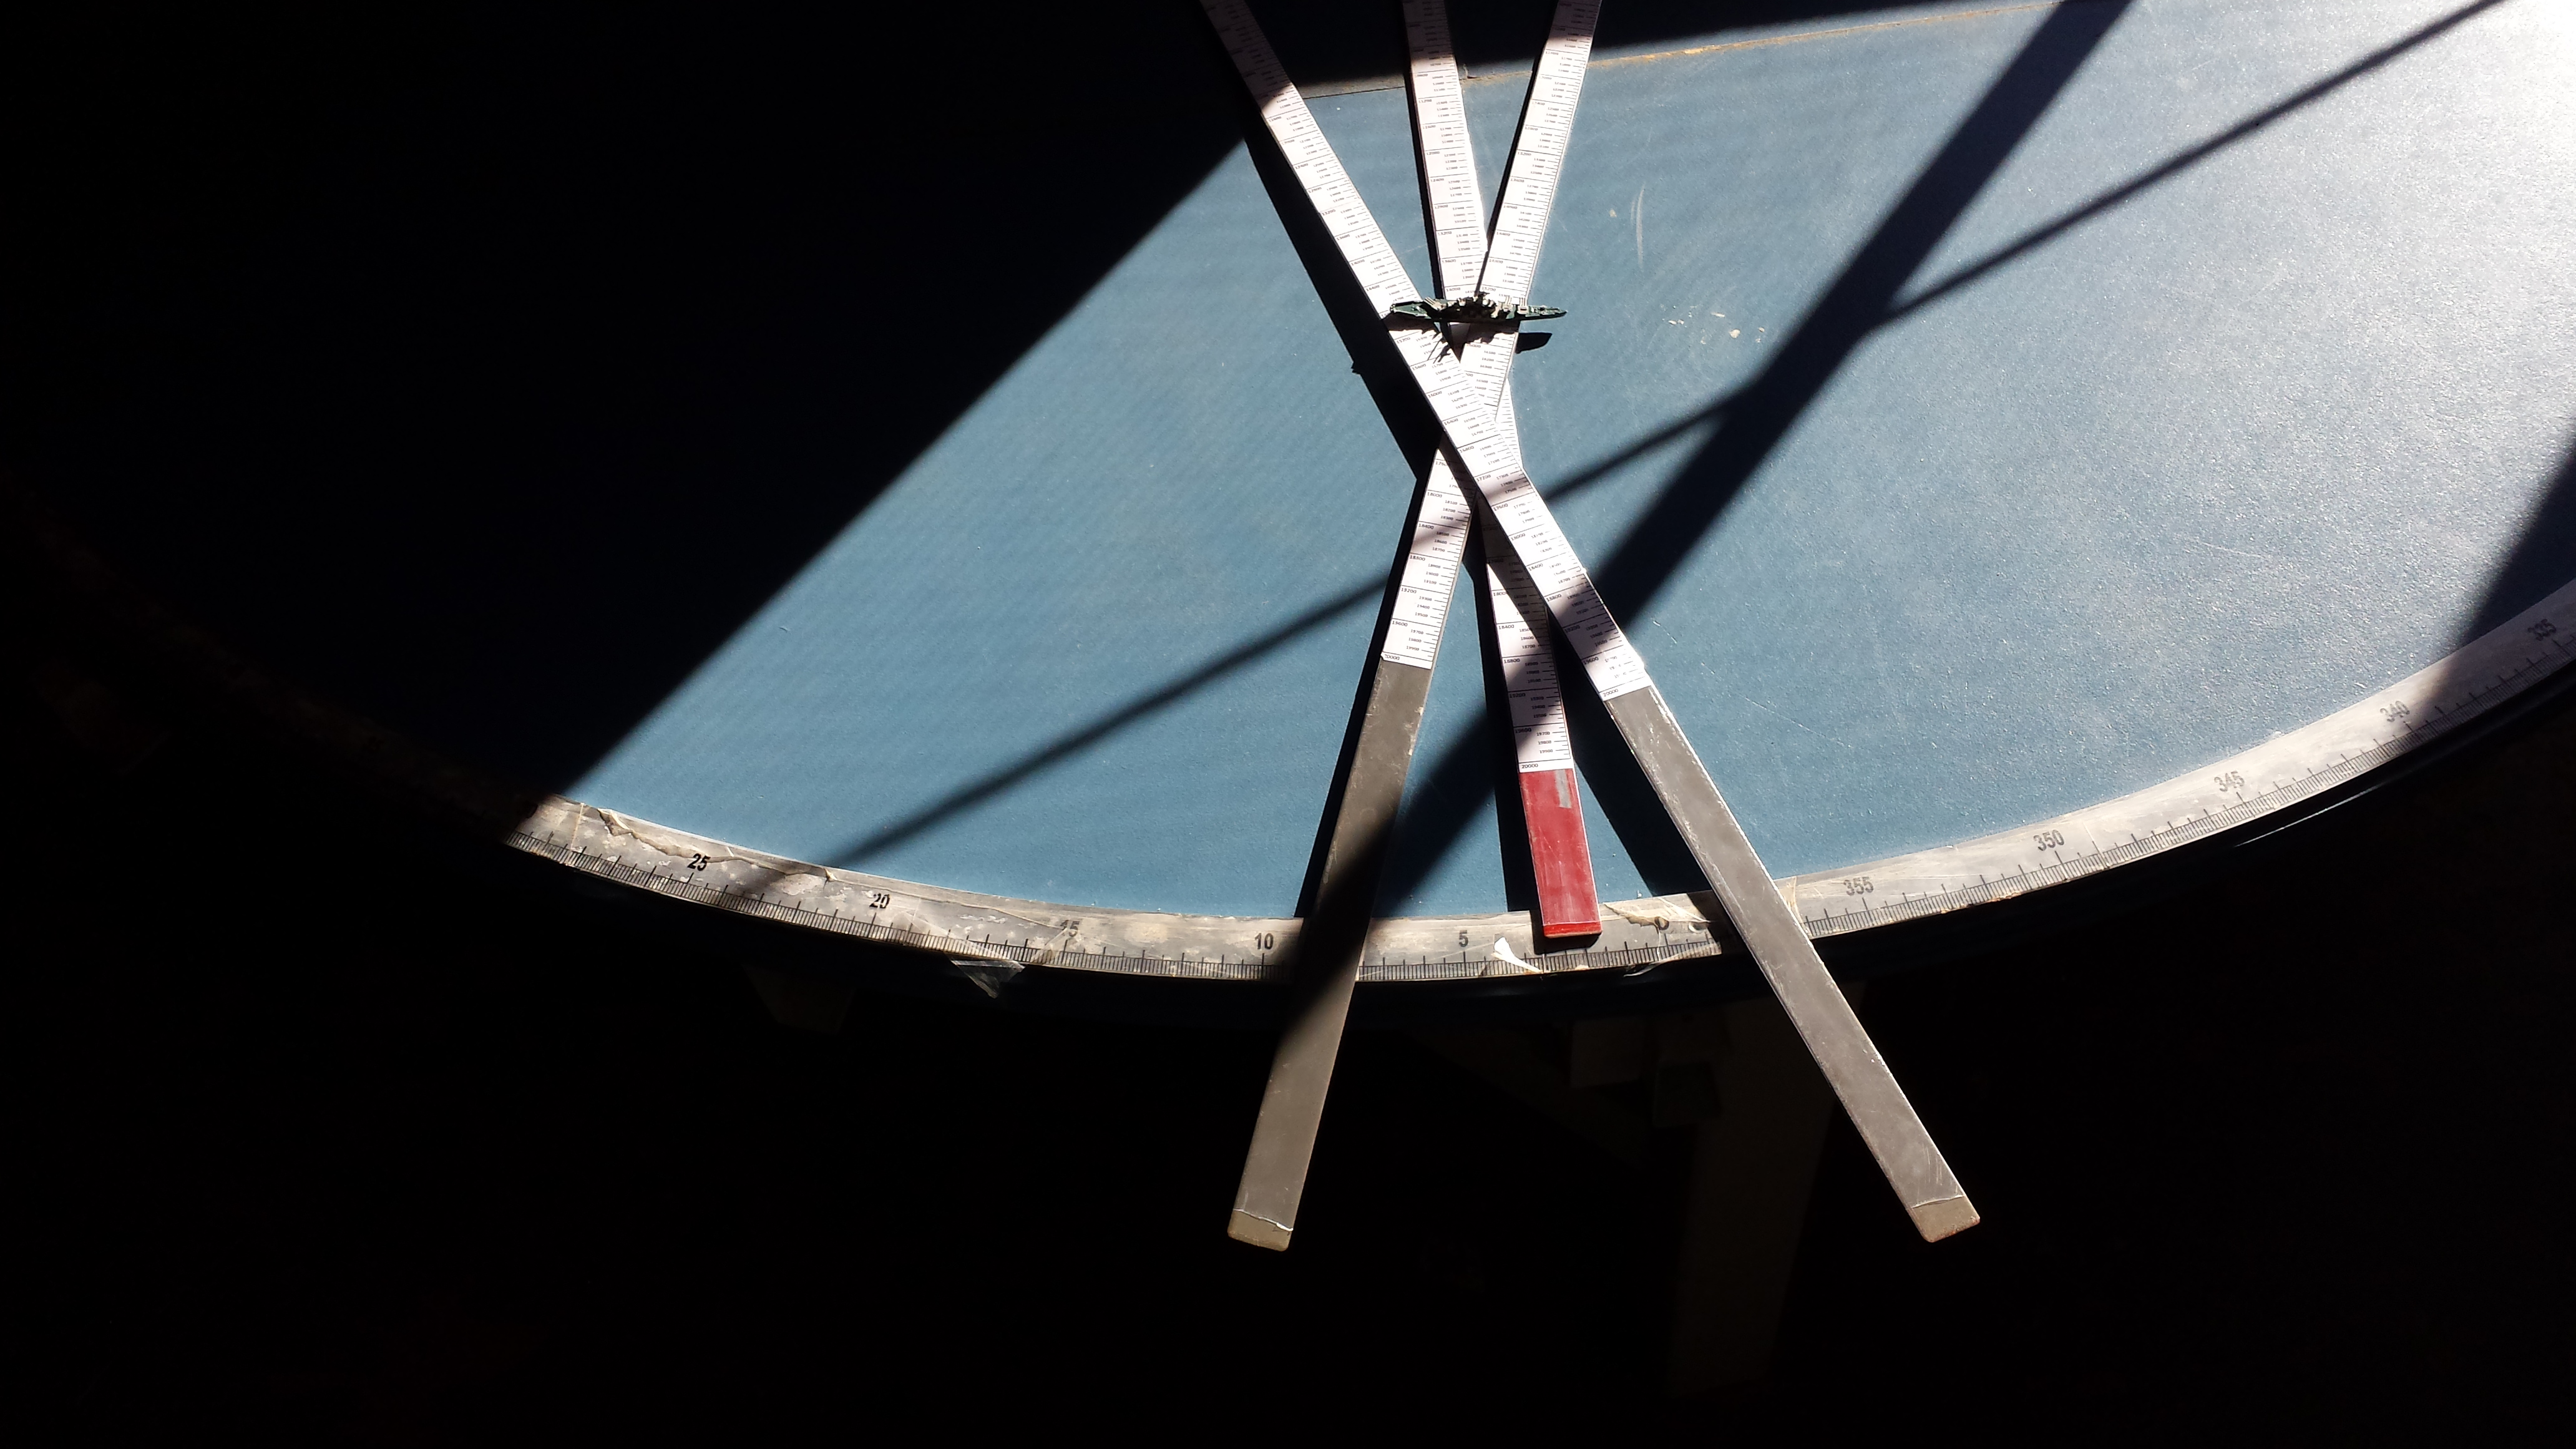
\includegraphics[width=0.5\textwidth]{test_image.jpg}
  \caption{I can embed images too}
\end{figure}

\noindent
We can make a table with centered elements:

\vspace{5mm}
\[ \left[ \begin{array}{c c c}
1.1754 & -0.8334 & 193.4191\\
0.2062 & 1.0380 & -141.0333\\
-0.0008 & 0.0007 & 1.0000\\
\end{array}
\right] \]
\vspace{5mm}

\noindent
There you go! That should be enough to get you started on LaTeX!

\end{document}
